\begin{figure}
	\centering
	\pgfplotsset{every axis legend/.append style={
		at={(1.05,0.5)},
		anchor=west}}
	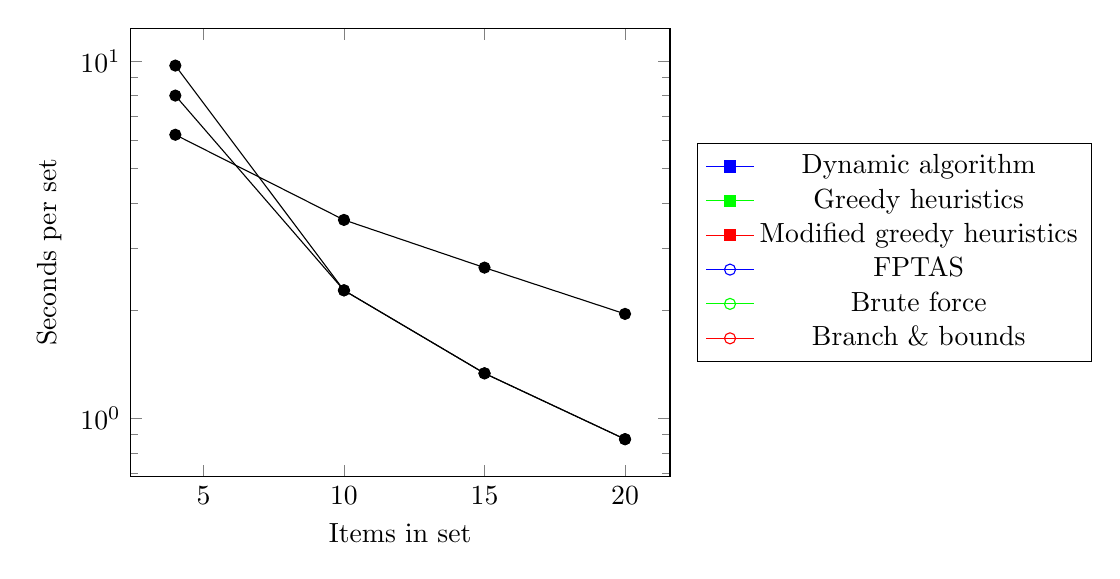
\begin{tikzpicture}
		\begin{semilogyaxis}[
			xlabel=Items in set,
			ylabel=Seconds per set,
			scatter/classes={
				solvePriceDynamic={mark=square*,blue},
				solveHungry={mark=square*,green},
				solveSingle={mark=square*,red},
				fptas={mark=o,blue},
				solveStupid={mark=o,green},
				solveSmart={mark=o,red}
				}
            ]
            
\addplot[scatter,scatter src=explicit symbolic]table[meta=label] {
x y label
4 9.701940 hungryStupidDeviation
10 2.280480 hungryStupidDeviation
15 1.336278 hungryStupidDeviation
20 .874248 hungryStupidDeviation
};
\addplot[scatter,scatter src=explicit symbolic]table[meta=label] {
x y label
4 7.997880 singleDeviation
10 2.280480 singleDeviation
15 1.336278 singleDeviation
20 .874248 singleDeviation
};
\addplot[scatter,scatter src=explicit symbolic]table[meta=label] {
x y label
4 6.213740 fptasDeviation
10 3.590200 fptasDeviation
15 2.640060 fptasDeviation
20 1.959616 fptasDeviation
};

			\addlegendentry{Dynamic algorithm}
			\addlegendentry{Greedy heuristics}
			\addlegendentry{Modified greedy heuristics}
			\addlegendentry{FPTAS}
			\addlegendentry{Brute force}
			\addlegendentry{Branch \& bounds}
		\end{semilogyaxis}
	\end{tikzpicture}
\caption{Average time per set with weak correlation}
\label{plot:correlationWeakTime}
\end{figure}
